\section{Fibre and Fabric: Understanding the Distinction}

In textile production, both "fibre" and "fabric" terms are commonly used. Fibre and fabric are both related, but they represent different steps in the creation of textiles. Knowing the differences between fibres and fabrics is important to understand the basic mechanisms of the textile manufacturing process and the characteristics of the final product.

\subsection{Fibre}

A \textbf{fibre} is the most basic building block of any textile material. It is a thin, thread of filament or a natural or man-made substance that is much longer than it is width. These individual filaments incorporate the inherent attributes that characterize the textile. The principal function of fibres is to be spun into a yarn; that yarn is then used to produce fabric \cite{researchgate}.

\textbf{Key characteristics of fibres:}
\begin{itemize}
    \item \textbf{Fundamental Unit:} Fibres are the smallest and most elementary components from which textiles are formed.
    \item \textbf{Filamentary Structure:} They possess a slender, elongated, and thread-like shape.
    \item \textbf{Source:} Fibres can be natural (e.g., obtained from plants like cotton, linen, jute; from animals like wool, silk) or synthetic (e.g., polyester, nylon, acrylic) \cite{researchgate}.
    \item \textbf{Properties:} The properties of a fibre (e.g., strength, elasticity, absorbency, softness, insulation) is a direct extension of the properties of used fibres as they influence the properties of the yarn and final fabric \cite{researchgate}.
    \item \textbf{Not directly usable as clothing:}  Fibres are usually too fine and short (staple fibres, e.g., cotton) or too weak (continuous filaments, e.g., silk before twist) to use individually in the construction of garments or most textile products. Fibres must be processed into yarn before being used \cite{researchgate}.
\end{itemize}

\textbf{Examples of Fibres:}
\begin{itemize}[noitemsep, topsep=0pt]
    \item \textbf{Natural:} Cotton, Linen, Jute, Wool, Silk, Hemp.
    \item \textbf{Synthetic:} Polyester, Nylon, Rayon, Spandex (Lycra), Acrylic.
\end{itemize}

\subsection{Fabric}

A \textbf{fabric} is, on the other hand, the material derived from interlacing, looping or otherwise bonding fibres or yarns together. Fabric is a more dense and cohesive material and may be used directly with minimal processing to produce clothing, home furnishings, industrial products, and a wide range of textile-based types of goods. Fabric is the result of several processes that convert raw fibres or yarns to attached or laminated fibres or yarns in sheet form \cite{researchgate, hong2024research}.

\textbf{Key attributes of fabrics:}
\begin{itemize}
    \item \textbf{Constructed Material:} Fabrics are the assembled arrangement of fibres or more often yarns. 
    \item \textbf{Methods of Construction:} Some of the methods that are commonly employed for making textiles are: 
        \begin{itemize}
            \item \textbf{Weaving:} The process (warp and weft) of interlacing two systems of yaml at right angles to one another forming a stable structure.
            \item \textbf{Knitting:} The interlooping of a single type of yarn can produce a warm, flexible stretching-yarn material.
            \item \textbf{Felting:} A process that may employ heat, moisture and friction where the fibres (usually wool) are pressed and then matted together to bind them to produce a dense solid nonwoven textile material.
            \item \textbf{Non-woven:} A process that provides some type of bonding (chemical, mechanical or thermal) of fibres without going through a spinning operation or weaving/knitting operation \cite{hong2024research}.
        \end{itemize}
        \item \textbf{Directly Usable:} Fabrics are completed textile materials both cut, sewn or finished to use in garment or product production.
        \begin{figure}[H]
            \centering
            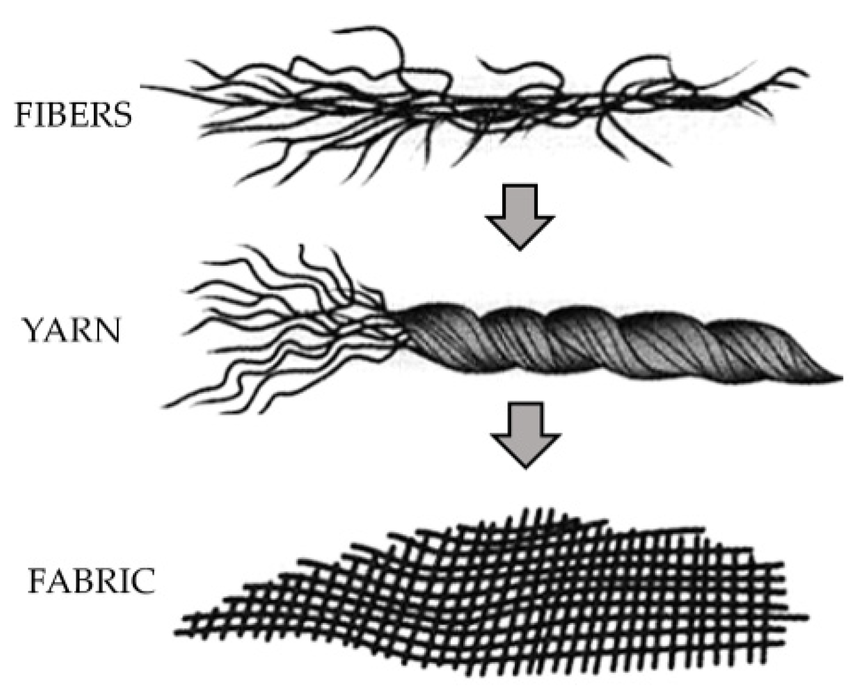
\includegraphics[width=0.6\textwidth]{images/fabric_construction}
            \caption{Construction of Fabric from Fibres}
            \label{fig:fabric_construction}
        \end{figure}
    \item \textbf{Properties derived from fibres and construction:} The properties of a fabric (e.g., drape, hand, durability, breathability, warmth) are determined by the fibres from which the yarn(s) are made, the fibres or yarns used, and the method used to construct the fabric (woven, knitted, etc.) \cite{researchgate, hong2024research}.
\end{itemize}

\textbf{Examples of Fabrics:}
\begin{itemize}[noitemsep, topsep=0pt]
    \item Cotton fabric, Silk fabric, Wool fabric, Polyester fabric, Denim, Chiffon, Fleece, Canvas.
\end{itemize}

\subsection{Differences between Fibre and Fabric}

It is necessary to remember that the textile industry is based upon the transformation process that connects fibre and fabric, to have context for the comparison. This transformation process takes raw materials through many different steps to turn them into functional and aesthetic products through a convoluted process of spinning, weaving, knitting, or bonding, etc. Designers, producers, and consumers must all acknowledge the fundamental connection between fibre and fabric, which demonstrates how raw materials are transformed into textiles we regularly use in our daily lives for apparel, furnishings, and other items. The table below segments their differences based on their roles and characteristics in textile processes.

\newpage

\begin{table}[h!]
    \centering
    \caption{Key differences between Fibre and Fabric}
    \label{tab:fibre_fabric_diff}
    \begin{tabular}{l p{5cm} p{5cm}} % Adjust column width for content
        \toprule
        \textbf{Feature} & \textbf{Fibre} & \textbf{Fabric} \\
        \midrule
        \textbf{Definition} & A single, thread-like filament or natural/synthetic substance \cite{researchgate}. & A material produced by weaving, knitting, felting, or bonding fibres/yarns \cite{researchgate, hong2024research}. \\
        \textbf{Form} & Basic, raw, individual component. & Constructed, cohesive, sheet-like material. \\
        \textbf{Stage of Production} & Precursor to yarn. The fundamental unit. & End product of textile formation (from yarn/fibre). \\
        \textbf{Usability} & Not directly used for clothing/products (must be processed) \cite{researchgate}. & Directly usable for making clothing and other textile products. \\
        \textbf{Properties} & Determines inherent characteristics (e.g., raw strength, absorbency) \cite{researchgate}. & Properties result from fibre type \textit{and} construction method (e.g., drape, texture, finished strength) \cite{researchgate, hong2024research}. \\
        \textbf{Analogy} & Think of individual strands of hair. & Think of a piece of cloth woven from those hair strands. \\
        \bottomrule
    \end{tabular}
\end{table}

In short, fibres are raw ingredients, fabrics are the cooked meal, ready to be consumed (or in this case, made into garments). The process from multiple single adjustments of fibres, to a usable, textured fabric, involves significantly complex processes which define the aesthetic, tactile, and functional qualities of the final textile product.